\documentclass[11pt,letterpaper]{article}
\usepackage[lmargin=1in,rmargin=1in,bmargin=1in,tmargin=1in]{geometry}
\usepackage{style/quiz}
\usepackage{style/commands}

% Logical Circuits
\usepackage{circuitikz}
\usetikzlibrary{shapes.gates.logic.US,shapes.gates.logic.IEC}

% -------------------
% Content
% -------------------
\begin{document}
\thispagestyle{title}

% Quiz 1
\quizsol \textit{True/False}: The expression $P \to Q$ is logically equivalent to $\neg P \vee Q$. \pspace

\sol The statement is \textit{true}. One method of seeing is this is to compute the truth table for $P \to Q$ and $\neg P \vee Q$ and see that the outputs of $P \to Q$ and $\neg P \vee Q$ match, no matter the inputs for $P, Q$. \par
	\begin{table}[h]
	\centering
	\begin{tabular}{ccccc}
	$P$ & $Q$ & $P \to Q$ & $\neg P$ & $\neg P \vee Q$ \\ \hline 
	$T$ & $T$ & $\mathbf{T}$ & $F$ & $\mathbf{T}$ \\
	$T$ & $F$ & $\mathbf{F}$ & $F$ & $\mathbf{F}$ \\
	$F$ & $T$ & $\mathbf{T}$ & $T$ & $\mathbf{T}$ \\
	$F$ & $F$ & $\mathbf{T}$ & $T$ & $\mathbf{T}$
	\end{tabular}
	\end{table} \par
As we can see, the third and fourth columns corresponding to $P \to Q$ and $\neg P \vee Q$, respectively, are the same, $P \to Q \equiv \neg P \vee Q$. Alternatively, $P \to Q$ will be logically equivalent to $\neg P \vee Q$ if they are always simultaneously true. We know for $P \to Q$ to be true, either $P$ must be false or $P, Q$ must both be true. Observe that if $P$ is false, then $\neg P$ is true so that $\neg P \vee Q$ is true. If $P, Q$ are true, then $\neg P \vee Q$ is true. Loosely, $P \to Q$ is true if either $P$ does not occur or if $Q$ occurs. But this is precisely $\neg P \vee Q$. In any case, it is true that $P \to Q \equiv \neg P \vee Q$. \pvspace{1.3cm}



% Quiz 2
\quizsol \textit{True/False}: The logical expression corresponding to the circuit below is $\neg (P \wedge Q) \wedge (P \vee \neg Q)$
	\[
	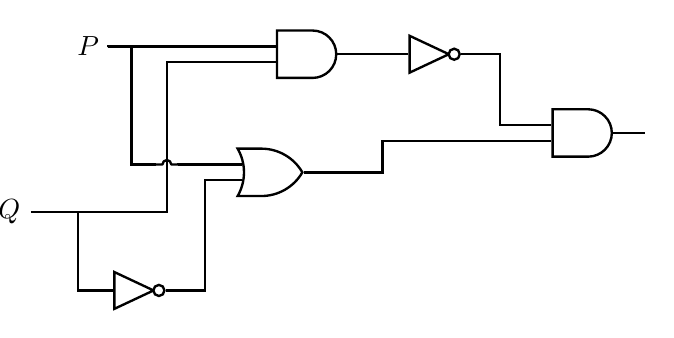
\begin{tikzpicture}
	\node (p) at (0,2.1) {\hspace{-0.5cm}$P$};
	\node (q) at (-1,0) {\hspace{-0.5cm}$Q$};
	
	\node[and gate US, draw, line width= 0.03cm] at (2.5,2) (and1) {};
	\node[not gate US, draw, line width= 0.03cm] at (4,2) (not1) {};
	\node[not gate US, draw, line width= 0.03cm] at (0.25,-1) (not2) {};
	\node[or gate US, draw, line width= 0.03cm] at (2,0.5) (or1) {};
	\node[and gate US, draw, line width= 0.03cm] at (6,1) (and2) {};
	
	\draw[line width= 0.03cm] (p) |- (and1.input 1);
	\draw[line width= 0.03cm] (and1.output) |- (not1.input);
	\draw[line width= 0.03cm] (not1.output) -- ([xshift=0.5cm]not1.output) |- (and2.input 1);
	\draw[line width= 0.03cm] (q) -- (0.75,0) |- (and1.input 2);
	\draw[line width= 0.03cm] (-0.375,0) |- (not2.input);
	\draw[line width= 0.03cm] (not2.output) -- ([xshift=0.5cm]not2.output) |- (or1.input 2);
	\draw[line width= 0.03cm] (or1.output) -- ([xshift=1cm]or1.output) |- (and2.input 2);
	\draw[line width= 0.03cm] (and2.output) -- ([xshift=0.4cm]and2.output);	
	\draw[line width= 0.03cm] (0.3,2.1) -- (0.3,0.6) -- (0.6,0.6) to[crossing] (0.9,0.6) |- (or1.input 1);
	\end{tikzpicture}
	\]

\sol The statement is \textit{true}. To see this, we can follow the circuit, labeling the wires as we go. 
	\[
	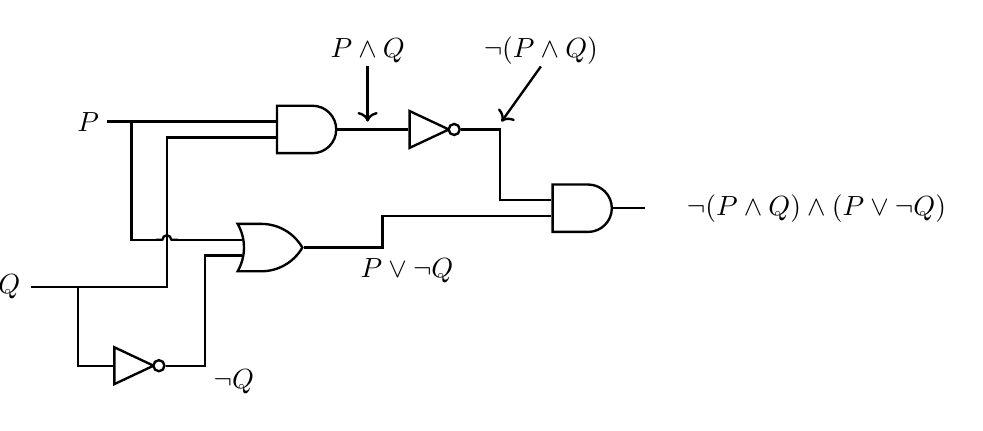
\begin{tikzpicture}
	\node (p) at (0,2.1) {\hspace{-0.5cm}$P$};
	\node (q) at (-1,0) {\hspace{-0.5cm}$Q$};
	
	\node[and gate US, draw, line width= 0.03cm] at (2.5,2) (and1) {};
	\node[not gate US, draw, line width= 0.03cm] at (4,2) (not1) {};
	\node[not gate US, draw, line width= 0.03cm] at (0.25,-1) (not2) {};
	\node[or gate US, draw, line width= 0.03cm] at (2,0.5) (or1) {};
	\node[and gate US, draw, line width= 0.03cm] at (6,1) (and2) {};
	
	\draw[line width= 0.03cm] (p) |- (and1.input 1);
	\draw[line width= 0.03cm] (and1.output) |- (not1.input);
	\draw[line width= 0.03cm] (not1.output) -- ([xshift=0.5cm]not1.output) |- (and2.input 1);
	\draw[line width= 0.03cm] (q) -- (0.75,0) |- (and1.input 2);
	\draw[line width= 0.03cm] (-0.375,0) |- (not2.input);
	\draw[line width= 0.03cm] (not2.output) -- ([xshift=0.5cm]not2.output) |- (or1.input 2);
	\draw[line width= 0.03cm] (or1.output) -- ([xshift=1cm]or1.output) |- (and2.input 2);
	\draw[line width= 0.03cm] (and2.output) -- ([xshift=0.4cm]and2.output);	
	\draw[line width= 0.03cm] (0.3,2.1) -- (0.3,0.6) -- (0.6,0.6) to[crossing] (0.9,0.6) |- (or1.input 1);
	
	\draw[line width=0.03cm,->] (3.3,2.8) -- (3.3,2.1);
	\node at (3.3,3) {$P \wedge Q$};
	\draw[line width=0.03cm,->] (5.5,2.8) -- (5,2.1);
	\node at (5.5,3) {$\neg (P \wedge Q)$};
	\node at (1.6,-1.2) {$\neg Q$};
	\node at (3.8,0.2) {$P \vee \neg Q$};
	\node at (9,1) {$\neg (P \wedge Q) \wedge (P \vee \neg Q)$};
	\end{tikzpicture}
	\]



\newpage



% Quiz 3
\quizsol \textit{True/False}: Let $\mathcal{U}$ be the set of integers. Consider the predicate $P(n) \colon n^2 + 5 > 20$. Because $P(5)$ is true, we know that both $\exists n\, P(n)$ and $\forall n\, P(n)$ are true. \pspace 

\sol The statement is \textit{false}. Because $P(5) \colon 5^2 + 5= 25 + 5= 30 > 20$ is true, we know there exists an integer $n$---for example $n= 5$---such that $P(n)$ is true. Therefore, $\exists n \, P(n)$ is true. However, the statement $\forall n \, P(n)$ need not be true simply because there is an $n$ such that $P(n)$ is true. For example, $P(1) \colon 1^2 + 5= 1 + 5= 6 \not> 20$. But because $P(n)$ is not true when $n= 1$, the predicate $P(n)$ is not true for all $n$. Therefore, $\forall n\, P(n)$ is false. But then the claim that both $\exists n\, P(n)$ and $\forall n\, P(n)$ are true is false. \pvspace{1.3cm}



% Quiz 4
\quizsol \textit{True/False}: If $P(x)$ is a predicate with nonempty universe $\mathcal{U}$, then there are values of $x$ for which $P(x)$ is true, and there are values for which $P(x)$ is false. \pspace

\sol The statement is \textit{false}. If $P(x)$ is a predicate with universe $\mathcal{U}$, then one of the following must be true: $P(x)$ is true for all $x \in \mathcal{U}$, $P(x)$ is false for all $x \in \mathcal{U}$, or there are values $x, y \in \mathcal{U}$ such that $P(x)$ is true and $P(y)$ is false. Each possibility occurs. For instance, let the universe $\mathcal{U}$ be the set of real numbers. If $P(x)$ is the predicate $P(x) \colon x^2 \geq 0$, then $P(x)$ is true for all $x \in \mathcal{U}$. If $P(x)$ is the predicate $P(x) \colon x^2 < 0$, then $P(x)$ is false for all $x \in \mathcal{U}$. If $P(x)$ is the predicate $P(x) \colon x^2 > 1$, then $P(1) \colon 1^2 = 1 \not> 1$, i.e. $P(1)$ is false, while $P(2) \colon 2^2= 4 > 1$ is true, i.e. $P(2)$ is true. But then it is not true that for a given predicate $P(x)$ nonempty universe $\mathcal{U}$, there are values of $x$ for which $P(x)$ is true, and there are values for which $P(x)$ is false. \pvspace{1.3cm}



% Quiz 5
\quizsol \textit{True/False}: Let $S= \{ x \in \mathbb{Z} \colon (2x - 1)(x + 6)= 0 \}$. The set $S$ has infinitely many elements; in particular, the set $S$ is nonempty. \pspace

\sol The statement is \textit{false}. Suppose that $s \in S$. Then $s \in \mathbb{Z}$ and $(2s - 1)(s + 6)= 0$. But this implies $2s - 1=0$ or $s + 6= 0$, which in turn implies $s= \frac{1}{2}$ or $s= -6$. Because $s \in \mathbb{Z}$, we know that $s \neq \frac{1}{2}$. It must then be that if $s \in S$, $s= -6$. We can verify that $s \in S$: $-6 \in \mathbb{Z}$ and $(2 \cdot -6 - 1)(-6 + 6)= -5 \cdot 0= 0$. This shows that $S= \{ -6 \}$; therefore, $S$ is nonempty. However, clearly $S$ is not infinite. Therefore, the statement of the quiz is false. \pvspace{1.3cm}



% Quiz 6
\quizsol \textit{True/False}: If $S= \varnothing$, then $\mathcal{P}(S)= \varnothing$. \pspace

\sol The statement is \textit{false}. We know that for any set $S$, $\mathcal{P}(S)$ is the set of subsets of $S$. For any set $S$, $\varnothing \subseteq S$ and $S \subseteq S$. Therefore, $\{ \varnothing, S \} \subseteq \mathcal{P}(S)$ for all sets $S$. But then we cannot have $\mathcal{P}(S)= \varnothing$. So the statement of the quiz is false. In fact, $\mathcal{P}(S)= \{ \varnothing \}$. 



\newpage



% Quiz 7
\quizsol \textit{True/False}: $\displaystyle \left( \bigcup_{n \in \mathbb{N}} [0, n) \right)^c= (-\infty, 0)$ \pspace

\sol The statement is \textit{true}. The union of a collection of sets is the set consisting of the elements in any of the sets in the collection. But then the union contains all of the elements of $[0, n)$ for all $n \in \mathbb{N}$. But then given a nonnegative real $x$, choose $n \in \mathbb{N}$ so that $x < n$. This shows $x \in [0, n) \subseteq \displaystyle \bigcup_{n \in \mathbb{N}} [0, n)$. If $x$ is a negative real, then $x \notin [0, n) \subseteq \displaystyle \left( \bigcup_{n \in \mathbb{N}} [0, n) \right)$ for all $n \in \mathbb{N}$. But this shows that $\displaystyle \left( \bigcup_{n \in \mathbb{N}} [0, n) \right)= [0, \infty)$. Therefore, we have\dots
	\[
	\displaystyle \left( \bigcup_{n \in \mathbb{N}} [0, n) \right)^c= [0, \infty)^c= (-\infty, 0)
	\]
Alternatively, we have\dots
	\[
	\displaystyle \left( \bigcup_{n \in \mathbb{N}} [0, n) \right)^c= \bigcap_{n \in \mathbb{N}} [0, n)^c= \bigcap_{n \in \mathbb{N}} \bigg( (-\infty, 0) \cup [n, \infty) \bigg)= (-\infty, 0) \cup \bigcap_{n \in \mathbb{N}} [n, \infty)
	\]
Clearly, if $x$ is a negative real, $x \notin [n, \infty)$ for all $n \in \mathbb{N}$, so that $x \notin \displaystyle \bigcap_{n \in \mathbb{N}} [n, \infty)$. If $x$ were a nonnegative real in $\displaystyle \bigcap_{n \in \mathbb{N}} [n, \infty)$, then $x \in [n, \infty)$ for all $n \in \mathbb{N}$. But again, choosing $n \in \mathbb{N}$ with $x < n$ shows that $x \notin [n, \infty)$. But then $x \notin \displaystyle \bigcap_{n \in \mathbb{N}} [n, \infty)$. But this shows\dots 
	\[
	\displaystyle \left( \bigcup_{n \in \mathbb{N}} [0, n) \right)^c= (-\infty, 0) \cup \bigcap_{n \in \mathbb{N}} [n, \infty)= (-\infty, 0) \cup \varnothing= (-\infty, 0)
	\]



%Let $A$ be the set of perfect squares. Let $f: A \to \mathbb{Z}$ be the relation given as follows: if $b$ is an integer such that $a= b^2$, then $f(a)= b$. The relation $f$ is a function. 
%Let $X, Y$ be sets and $f: X \to Y$ be a function. Then $f$ is surjective to its image; that is, defining $\widetilde{f}: X \to \text{im } f$ via $\widetilde{f}(x):= f(x)$ for all $x \in X$, the function $\widetilde{f}$ is onto. 
%Let $A, B, C$ be sets and $f: A \to B, g: B \to C$ be functions. If $f$ is not injective, then $g \circ f$ is \textit{never} injective. 
%If $A, B$ are $n \times n$ diagonal matrices, then $AB= BA$. 

























\end{document}